\subsection{Regularyzacja}
Zajmijmy się regularyzacją naszego zbioru danych. Podzielmy zbiór na zmienne objaśniające (\textbf{X}) i zmienną objaśnianą (\textbf{y}).

\begin{Rcode}
X <- model.matrix(Type_of_Renewable_Energy ~ ., data = energy_data)[, -1]
y <- energy_data$Type_of_Renewable_Energy
\end{Rcode}

\subsubsection{Regresja grzbietowa}
Rozpocznijmy regularyzację od przeprowadzenia regresji grzbietowej dla określonego ciągu \textbf{\lambda}

\begin{Rcode}
lambda_grid <- 10^seq(10, -2, length.out = 100)
fit_ridge <- glmnet(X, y, alpha = 0, lambda = lambda_grid)
\end{Rcode}

Zestaw estymat \textbf{fit\_ridge} to macierz o rozmiarch \textbf{13} (liczba kolumn) na \textbf{100} (długość lambda\_grid).

Sprawdźmy normy euklidesowe dla estymat:

\begin{Rcode}
fit_ridge$lambda[50]
coef_ridge <- coef(fit_ridge)[, 50]
coef_ridge
sqrt(sum(coef_ridge[-1]^2))
\end{Rcode}

Im większa wartość \textbf{lamba}, tym mniejsze wartości estymat współczynników.

TUTAJ WYKRES

Sprawdźmy to dla testowego MSE:

\begin{Rcode}
set.seed(1)
n <- nrow(X)
train <- sample(n, n / 2)
test <- -train
fit_ridge <- glmnet(X[train,], y[train], alpha = 0, lambda = lambda_grid,
                    thresh = 1e-12)
\end{Rcode}

Dla \(\boldsymbol{\lambda = 4}\):
\begin{Rcode}
pred_ridge <- predict(fit_ridge, s = 4, newx = X[test,])
mean((pred_ridge - y[test])^2)
\end{Rcode}
Średnia otrzymana wartość to 4.044904.


Dla \(\boldsymbol{\lambda = 10^{10}}\):
\begin{Rcode}
pred_ridge_big <- predict(fit_ridge, s = 1e10, newx = X[test,])
mean((pred_ridge_big - y[test])^2)
\end{Rcode}
Średnia otrzymana wartość to 4.043964.


Dla \(\boldsymbol{\lambda = 0}\), czyli po prostu dla \textbf{metody najmniejszych kwadrató}:
\begin{Rcode}
pred_ridge_0 <- predict(fit_ridge, x = X[train,], y = y[train], s = 0, 
                      newx = X[test,], exact = TRUE)
mean((pred_ridge_0 - y[test])^2)
\end{Rcode}
Średnia otrzymana wartość to 4.051379.

Porówwnajmy estematy współczynników:
\begin{Rcode}
lm(y ~ X, subset = train)
predict(fit_ridge, x = X[train,], y = y[train], s = 0, exact = TRUE, 
        type = "coefficients")[1:13,]
\end{Rcode}

\begin{figure}[H]
    \centering
    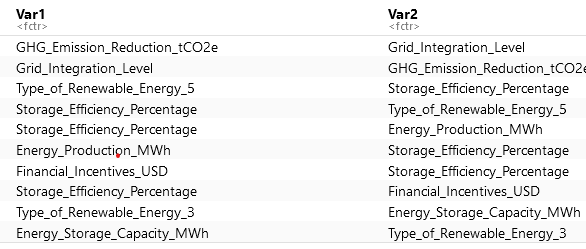
\includegraphics[width=1\linewidth]{lab4/obraz.png}
    \caption{Enter Caption}
    \label{fig:enter-label}
\end{figure}

Wyliczmy optymalne estymaty przy pomocy walidacji krzyżowej:

\begin{Rcode}
set.seed(1)
cv_out <- cv.glmnet(X[train,], y[train], alpha = 0)
plot(cv_out)
cv_out$lambda.min
\end{Rcode}

\begin{figure}[H]
    \centering
    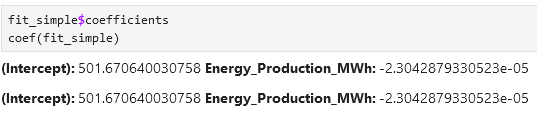
\includegraphics[width=1\linewidth]{lab4/obraz2.png}
    \caption{Enter Caption}
    \label{fig:enter-label}
\end{figure}

Otrzymaliśmy optymalną wartość $\lambda = 7.788007$. MSE dla takiej wartości wynosi 4.04435.

Estymaty współczynników dla optymalnej wartości $\lambda$:

\begin{figure}[H]
    \centering
    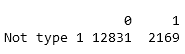
\includegraphics[width=1\linewidth]{lab4/obraz3.png}
    \caption{Intercept to estymata przy objaśnianiu zmiennej nią samą}
    \label{fig:enter-label}
\end{figure}

\subsubsection{Lasso}
Teraz spróbujemy wykorzystać metodę \textbf{L}east \textbf{A}bsolute \textbf{S}hrinkage and \textbf{S}election \textbf{O}perator - \textbf{LASSO}.

Dopasujmy LASSO do parametrów:

\begin{Rcode}
fit_lasso <- glmnet(X[train,], y[train], alpha = 1)
\end{Rcode}

\begin{figure}[H]
    \centering
    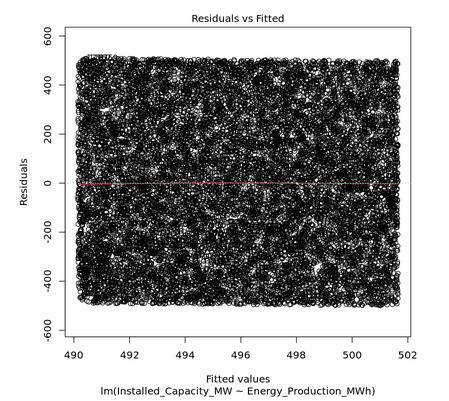
\includegraphics[width=1\linewidth]{lab4/obraz4.png}
    \caption{Enter Caption}
    \label{fig:enter-label}
\end{figure}

Wykonujemy walidację krzyżową i liczymy estymatę MSE:

\begin{Rcode}
cv_out <- cv.glmnet(X[train,], y[train], alpha = 1)
plot(cv_out)
cv_out$lambda.min
pred_lasso <- predict(fit_lasso, s = cv_out$lambda.min, newx = X[test,])
mean((pred_lasso - y[test])^2)
\end{Rcode}

\begin{figure}[H]
    \centering
    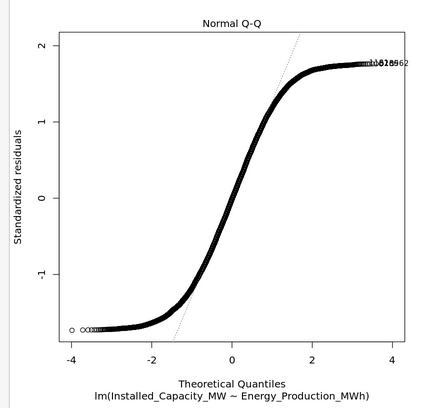
\includegraphics[width=1\linewidth]{lab4/obraz5.png}
    \caption{Enter Caption}
    \label{fig:enter-label}
\end{figure}

Otrzymaliśmy MSE na poziomie \textbf{4.04522} - wynik trochę słabszy niż przy regresji grzbietowej.

\textbf{DODAJ WIĘCEJ PORÓWNAŃ}

Estymaty:
POPRAW

\subsection{Modele nieliniowe}
\subsubsection{Regresja wielomianowa}
\subsubsection{Regresja logistyczna wielomianowa}
\subsubsection{Funkcje schodkowe}
\subsection{Funkcje sklejane}
\subsubsection{Naturalne funkcje sklejane}
\subsubsection{Wygładzające funkcje sklejane}
\subsection{Regresja lokalna}
\subsection{Uogólnione modele addytywne (GAMs)}
\subsection{GAM w GLM}